% FIGURE PARALLELE
\begin{figure}[!ht]
\begin{center}
    \fbox{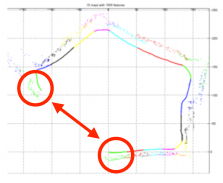
\includegraphics[width=.4\textwidth]{images/MobiDEV/lezione5/slam1.PNG}}
    \qquad \fbox{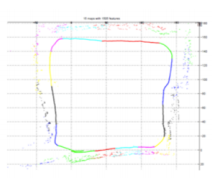
\includegraphics[width=.4\textwidth]{images/MobiDEV/lezione5/slam2.PNG}}
\end{center}
\end{figure}

% FIGURA ACCANTO AL TESTO
\begin{minipage}{.4\textwidth}
   Possiamo definire il problema in modo più generale considerando che per ogni oggetto $O_i$ conosco una distanza minima e massima rispetto ad x
\end{minipage} 
\hfill
\begin{minipage}{.6\textwidth}
    \begin{center}
        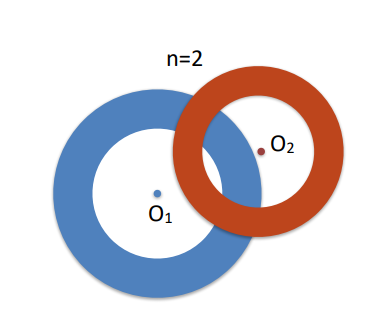
\includegraphics[width=.45\textwidth]{images/Mobile computing/4. Posizione/range di distanza.PNG}
    \end{center}
\end{minipage}

% IMMAGINE 
\begin{center}
    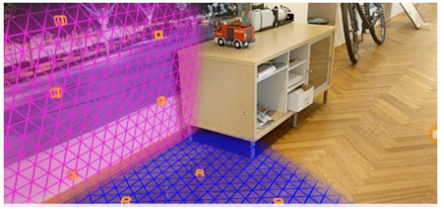
\includegraphics[width=.6\textwidth]{images/MobiDEV/lezione6/piano.PNG}
\end{center}

% TABELLA MULTILINEA
\begin{table}[!ht]
    \centering
    \begin{tabular}{p{.45\textwidth}|p{.45\textwidth}}
    \end{tabular}
    \caption{Caption}
    \label{tab:my_label}
\end{table}

% TABELLA CON TITOLO 
\begin{table}[!ht]
    \centering
    \begin{tabular}{|p{.4\textwidth}|p{.4\textwidth}|}
        \hline
        \multicolumn{2}{|c|}{\textbf{Lato server}} \\
        \hline
        \textbf{pro} & \textbf{contro}\\
        \hline
        
        \hline
    \end{tabular}
\end{table}